\chapter{High throughput (Multiple) QTL mapping}
\thispagestyle{empty}
\label{chap:mqm}

\emph{QTL mapping is the main analysis method used in the analysis of quantitative traits. This 
approach has been the analysis method to study quantitative traits since its discovery in 1980. 
Many variations to the basic single marker approach can be made, but none so fundamental as 
multiple QTL mapping using generalized lineair models. Computational and sample size problems 
were limiting the application of the approach. Novel experimental design and decreased costs 
have made sample size less of an issue, and by 'refreshing' the original algorithm more 
wide-spread application of this important algorithm is possible.}
\null
\vfill

\begin{myexampleblock}{Originally published as:}
  \authors{Danny Arends*, Pjotr Prins*, Ritsert C. Jansen and Karl W. Broman}\\
  \emph{R/qtl: High throughput Multiple QTL mapping}\\
  \bold{Bioinformatics} (2010) \\

  \authors{Danny Arends*, Ronny V. L. Joosen*, Leo Willems, Wilco Ligterink, Henk Hilhorst, Ritsert C. Jansen}\\
  Visualizing the genetic landscape of Arabidopsis seed performance\\
  \bold{Plant Physiology} (2011)\\

  \authors{Danny Arends*, Ronny V. L. Joosen*, Yang Li*, Leo Willems, Joost J.B. Keurentjes, Wilco Ligterink, 
  Ritsert C. Jansen, Henk Hilhorst}\\
  Identifying genotype-by-environment interactions in the metabolism of germinating Arabidopsis seeds using 
  Generalized Genetical Genomics\\
  \bold{Plant Physiology} (2013)
\end{myexampleblock}

\newpage

Here we show he contributions made to R/qtl and show the application of our newly developed toolset 
to map genetic variation underlying classical phenotypes in \emph{A. thalaina} seed development. We 
show that by using a reduced number of individuals using the designGG strategy we can map main- and 
interactioneffects with more statistical power compared to other designs. After this we use a limited 
number of individuals and continue our analysis by zooming into the metabolic level, we show that 
there are shared genetic loci between phenotypes at different bio-molecular levels. Additional using 
the new optimized MQM routine allows us to detect more loci and/or give more confidence in the loci 
detected.

\section{Single marker QTL mapping (R/qtl)}
R/qtl is an extensible, interactive environment for the mapping of quantitative trait loci (QTL) 
in experimental crosses. It is implemented as an add-on package for the freely available and 
widely used statistical language/software R \cite{R:2009}. Since its introduction, R/qtl 
\cite{Broman:2003} has become a reference implementation with an extensive guide on QTL mapping 
\cite{RQTLGuide:2009}. R/qtl development is continuous, with input from multiple collaborators 
and users.  We have introduced a full testing environment with regression testing, updated the 
license to the GPL version 3, and hosted the source code repository on Github, which gives R/qtl 
software development high visibility and transparency. 

The development of R/qtl reflects trends in quantitative genetics, in particular the use of 
larger datasets, larger calculations and requirements for controlling the false discovery rate. 
These developments are partly driven by high-throughput genetical genomics the name coined 
for the study of gene expression QTL (eQTL)\cite{Jansen:2001a}, metabolite QTL (mQTL), protein 
QTL (pQTL).

\section{Multiple QTL mapping}
Multiple QTL Mapping (MQM) belongs to a family of QTL mapping methods, that include Haley-Knott 
regression \cite{Haley:1992} and composite interval mapping CIM \cite{Zeng:1994}. MQM combines 
the strengths of generalized linear model regression with those of interval mapping 
\cite{Jansen:1993, Jansen:1994b}. 

Recent developments in QTL mapping include Bayesian modeling of multiple QTL e.g. R/qtlbim 
package \cite{Yandell:2007, Banerjee:2008}. Bayesian modeling, however, is computationally 
expensive, and arguably has little additional power when applied to high density maps, and 
(nearly) complete genotype data \cite{Handbook:Jansen:2007}. Still, we intend to combine the 
strengths of the different methods in future versions of R/qtl.

These days, with most experimental setups and high density maps, improving precision may be 
achieved by increasing the population size first. For more information on QTL mapping and 
Bayesian analysis we refer to the `Handbook of Statistical Genetics` \cite{Handbook:2007}. MQM 
makes used of generalized linear models, thereby potentially providing unified analysis of 
non-normal traits.

MQM provides a practical, relevant and sensitive approach for mapping QTL in experimental 
populations. The theoretical framework of MQM was introduced and explored by R.C. Jansen 
\cite{Jansen:1994a} and explained in the 'Handbook of Statistical Genetics' 
\cite{Handbook:Jansen:2007}. MQM has one known commercial implementation \cite{Mapqtl:2002}, 
which has been used effectively in practical research, resulting in hundreds of papers, e.g., 
in mouse, plant, and fish, respectively \cite{DeMooij:2009, Jeuken:2009, Kitano:2009}. Now, 
with MQM for R/qtl, we present the first free and open source implementation of MQM, that is 
multi-platform, scalable and suitable for automated procedures and large datasets.

\subsection{Features}
MQM for R/qtl is an automated three-stage procedure in which, in the first stage, missing 
genotype data is 'augmented'.  In other words, rather than guessing one likely genotype, 
multiple genotypes are modelled with their estimated probabilities. In the second stage, 
important marker cofactors are selected by multiple regression and backward elimination. 
The third stage, a QTL is moved along the chromosomes using these pre-selected markers as 
cofactors (Fig. \ref{fig:comparison}). QTL are interval-mapped using the most informative 
model selected by either maximum likelihood or restricted maximum likelihood. A refined 
and automated procedure for cases with large numbers of marker cofactors is included. 

\begin{figure}[h!]
  \centering
  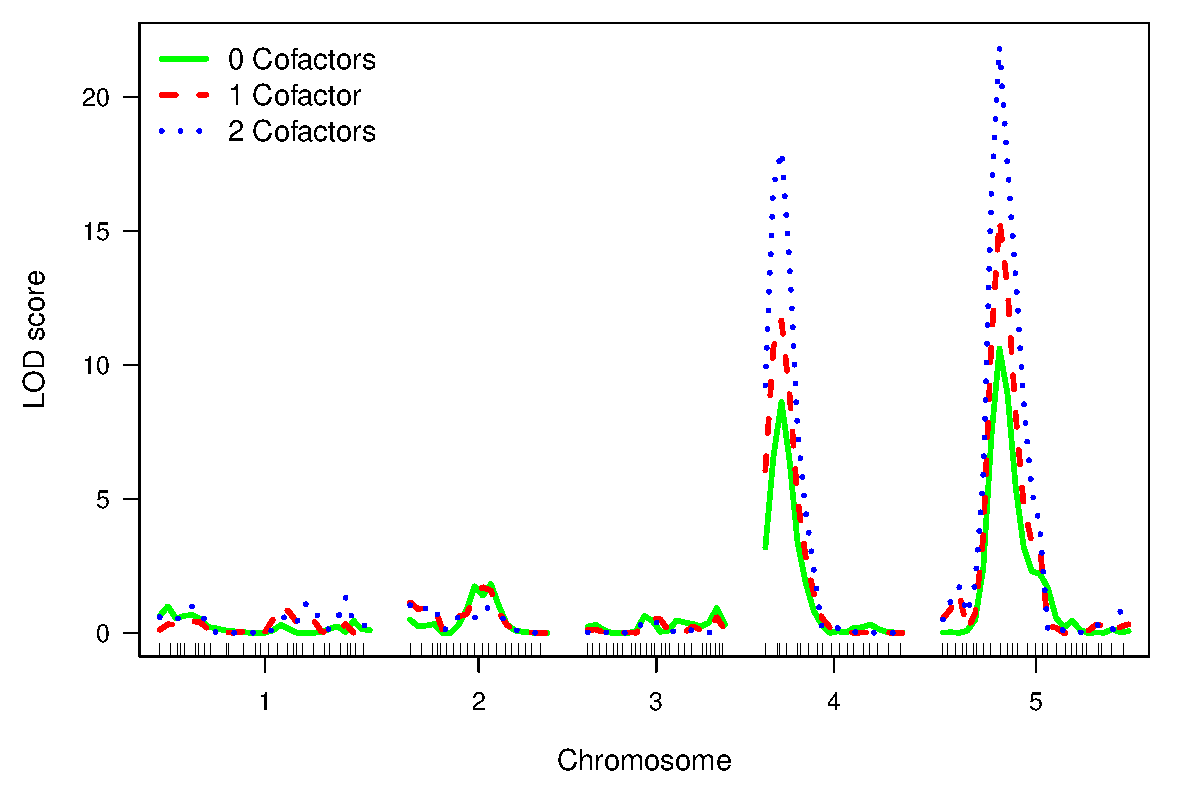
\includegraphics[keepaspectratio,scale=0.30]{eps/image_3_3.eps}
  \caption[Comparison of QTL mapping methodologies.]{ Three way comparison of MQM performance in {\it Arabidopsis 
          thaliana} \citep{Fu:2007}. LOD score increases when cofactors are added manually to the model. Here, 
          adding more than two cofactors does not improve the model any further (as discussed in the online 
          MQM tutorial).}
  \label{fig:comparison}
\end{figure}

The method lets users test different QTL models by elimination of non-significant cofactors. 
MQM for R/qtl brings the following advantages to QTL mapping:
\begin{enumerate}\itemsep1pt
\item Higher power, as long as the QTL explain a reasonable amount of variation.
\item Protection against over-fitting, because MQM fixes the residual variance from the full 
model, which allows the use of more cofactors than may be used in, for example, composite 
interval mapping \cite{Zeng:1994}.
\item Prevention of ghost QTL detection (between two QTL in coupling phase).
\item Detection of negating QTL (QTL in repulsion phase). 
\item MQM gives (compared to CIM) a reduction in type I and type II error \cite{Handbook:Jansen:2007}.
\item A pragmatic permutation strategy for controlling the false discovery rate (FDR) and 
prevention of locating false QTL hot spots, as discussed in Breitling et al \cite{Breitling:2008a}. 
Marker data is permuted, while keeping the correlation structure in the trait data.
\item High-performance computing by scaling on multi-CPU computers, as well as clustered 
computers, by calculating phenotypes in parallel, through the Message Passing Interface (MPI) of 
the SNOW package for R\cite{Tierney:2009}.
\item Visualizations for exploring interactions in a genomic circle plot (Fig. \ref{fig:circleplot}) and cis- 
and trans-regulation (Fig. \ref{fig:cistrans}).
\end{enumerate}

\begin{figure}[h!]
  \centering
  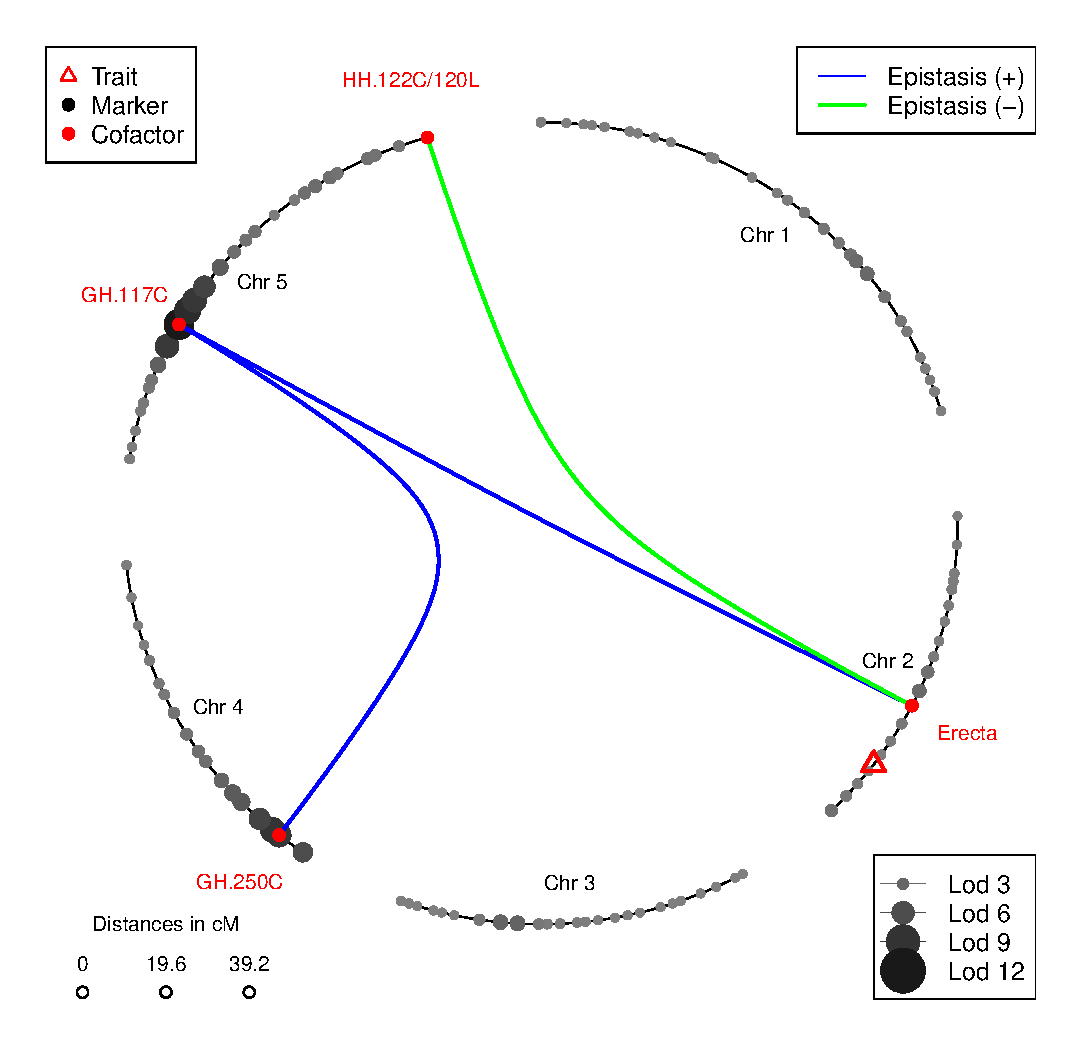
\includegraphics[keepaspectratio,scale=0.30]{eps/image_3_1.eps}
  \caption[Circle plot.]{Circular genome interaction plot \textcolor{black}{of the {\it Arabidopsis 
  		  thaliana} glucosinolate pathway} \citep{Fu:2007}.  LOD scores shown at marker positions 
  		  are scaled (grey circles), with selected cofactors (red circles) and epistasis between 
  		  multiple cofactors (green and blue splines)..}
  \label{fig:circleplot}
\end{figure}

\begin{figure}[h!]
  \centering
  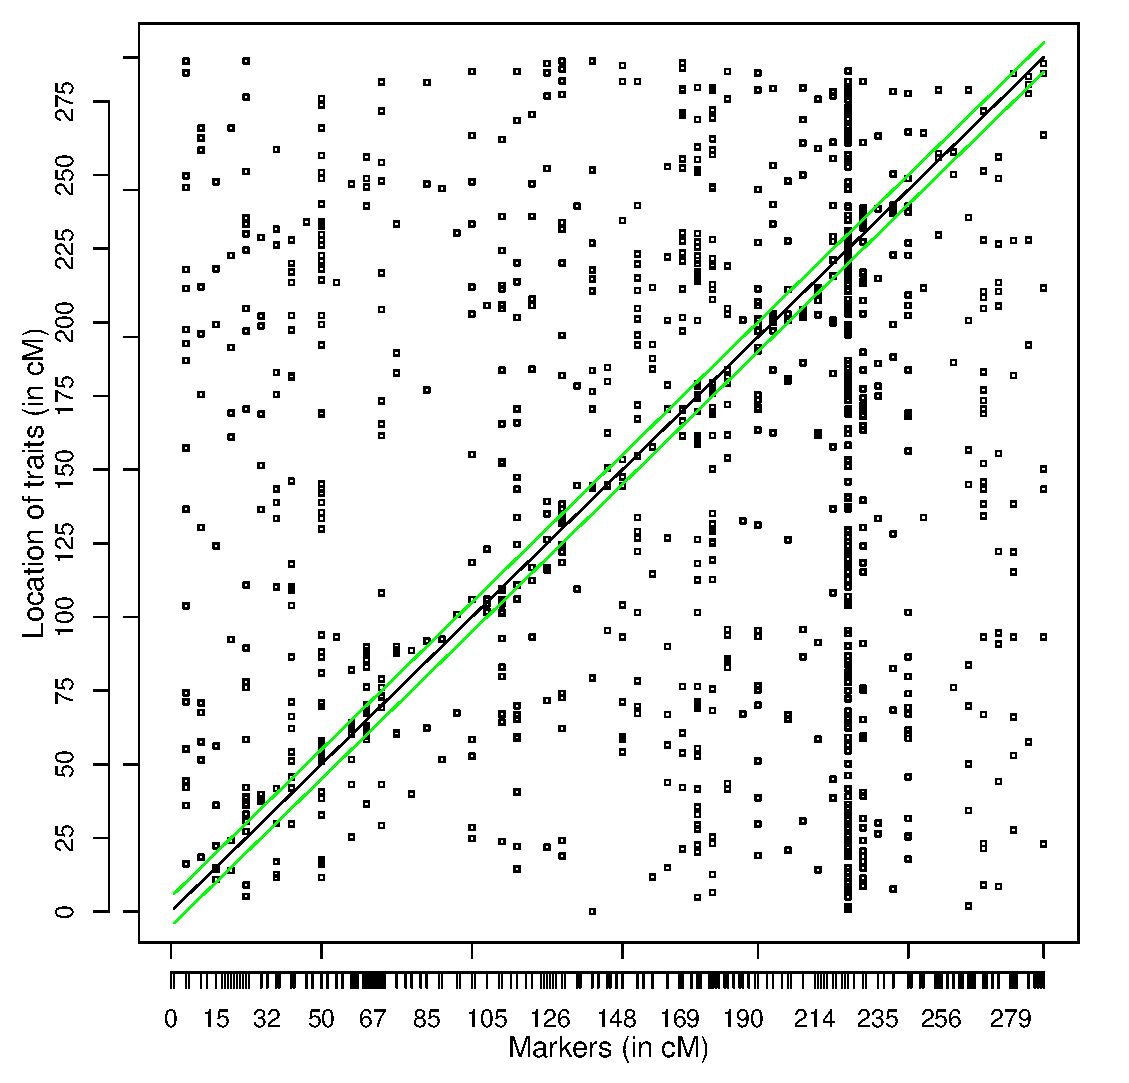
\includegraphics[keepaspectratio,scale=0.30]{eps/image_3_2.eps}
  \caption[CisTrans plot.]{Cis-trans plot of significant QTL (squares) showing cis acting QTL (diagonal) 
          and a trans-band (vertical, chromosome 5) in {\it Caenorhabditis elegans} \citep{Li:2006}.}
  \label{fig:cistrans}
\end{figure}

A 40-page tutorial for MQM explores, both the automated procedure, and the manual procedure 
of adding and removing cofactors, in an \emph{Arabidopsis thaliana} recombinant inbred line 
(RIL) metabolite (mQTL) dataset with 24 metabolites as phenotypes \cite{Fu:2007}. In addition, 
the tutorial visually explains the effects of data augmentation, cofactor selection, model 
selection, and tweaking of input parameters, such as cofactor significance. Genetic interactions 
(epistasis) are explored through effect plots, and an example is given of parallel computation. 
The tutorial is part of the software distribution of R/qtl and is available online.

\subsection{Conclusions and Discussion}
MQM for R/qtl is a significant addition to the QTL mapper's toolbox. R/qtl provides the user 
with the most frequently used statistical analysis methods: single-marker analysis, interval 
mapping, Haley-Knott regression \cite{Haley:1992}, CIM \cite{Zeng:1994} and MQM \cite{Jansen:1994a}. 
MQM has improved handling of missing data and allows more powerful and precise detection of QTL, 
compared to many other methods. Not only is this new implementation of MQM available in the
statistical R environment, which allows scripting for pipe-lined setups, it is also highly 
scalable through parallelisation and paves the way for high-throughput QTL analysis. With MQM, 
R/qtl is a free and high-performance comprehensive QTL mapping toolbox for the analysis of 
experimental populations. R/qtl now includes permutation strategies for determining thresholds 
of significance relevant for QTL and QTL hot spots; the first step towards causal inference and
network analysis.

